\فصل{مفاهیم اولیه}
در این فصل به بررسی برخی مفاهیم اولیه مورد نیاز در این پایان نامه پرداخته می‌شود.

\section{سرطان تیروئید}\label{sec:سرطان-تیروئید}
غده تیروئید یک غده پروانه‌ای شکل است که در قسمت تحتانی گردن قرار دارد.
این غده وظیفه کنترل متابولیسم و سوخت و ساز بدن را به عهده دارد.
علاوه بر این، تیروئید هورمون‌هایی تولید می‌کند که وظیفه تنظیم دمای بدن ، میزان سوخت و ساز و مصرف اکسیژن را انجام می‌دهد.
سرطان تیروئید زمانی رخ می‌دهد که سلول‌های غده تیروئید بر اثر عواملی، دچار تغییر می‌شوند و بعد از آن سلول‌های دارای ناهنجاری شروع به تکثیر می‌کنند و به تدریج تومور تیروئید را تشکیل می‌دهند.
سرطان تیروئید در صورتی که زودهنگام تشخیص داده شود یکی از قابل درمان‌ترین انواع سرطان است.

\subsection{انواع سرطان تیروئید}\label{subsec:انواع-سرطان-تیروئید}

سرطان تیروئید انواع مختلفی دارد که در هر کدام، ویژگی‌ها سلول متفاوت است.

\begin{itemize}
    \item سرطان پاپیلاری\LTRfootnote{Papillary Carcinomas}:
    این سرطان در ناحیه‌های کوچکی از بدن پخش می‌شود و حدود 80 درصد از نمونه سرطان‌های تیروئید رو تشکیل می‌دهد و در سلول های فولیکولی تولید کننده تیروگلوبولین در تیروئید شروع می شود.
    \item سرطان فولیکیولار\LTRfootnote{Follicular Carcinomas}:
    این نوع از سرطان در ناحیه بزرگتری از بدن و در زمان کمتری پخش می‌شود و حدود 15 درصد از نمونه سرطان‌های تیروئید رو تشکیل می‌دهد.
    \item سرطان مدولار\LTRfootnote{Medullary carcinoma}:
    این نوع از سرطان حدود 3 درصد از جمعیت کل بیماران سرطان غده تیروئید را تشکیل می‌دهد که از سلول های تولید کننده کلسی تونین در تیروئید ناشی می شود. 
    \item انواع نادر دیگر
\end{itemize}

هر کدام از انوع سرطان اشاره شده در قسمت اخیر را می توان با توجه به سطح خطری که آن‌ها برای بیماران دارند نیز دسته‌بندی کرد.
این دسته بندی مربوط به نوع سرطان تیروئید نیست و می‌توان سرطان‌های دیگری را نیز با این معیار دسته بندی کرد.
\begin{itemize}
    \item سرطان بدخیم\LTRfootnote{Malignant Carcinomas}:
    تومور بدخیم دارای مرزهای نامنظم است، سریعتر از یک تومور خوش‌خیم رشد می کند و می تواند به سایر قسمت های بدن شما نیز سرایت کند.
    \item سرطان خوش خیم\LTRfootnote{Benign Carcinomas}:
    تومور خوش‌خیم دارای مرزهای مشخص، صاف و منظم است، یک تومور خوش‌خیم می تواند بسیار بزرگ شود اما به بافت مجاور حمله نمی کند.
\end{itemize}
\subsection{روش‌های تشخیص سرطان تیروئید}\label{subsec:روش-های-تشخیص-سرطان-تیروئید}

برای تشخیص این سرطان روش‌های بسیاری وجود دارد.
از جمله این روش‌ها می‌توان به موارد زیر اشاره کرد.

\begin{itemize}
    \item معاینه فیزیکی:
    در این روش پزشک با معاینه بیمار به صورت فیزیکی و بررسی ناحیه تیروئید ممکن است متوجه غده سرطانی شود.
    \item سی تی اسکن\LTRfootnote{Computed tomography (CT) scan}:
    این آزمایش با استفاده از پرتوهای اشعه ایکس و به منظور تشخیص سایز و میزان انتشار تومورهای سرطانی تیروئید در سایر بخش‌های بدن انجام می‌شود.
    به طور مثال، اگر فردی مشکوک به سرطان تیروئید باشد، سی تی‌اسکن از ناحیه گردن و قفسه سینه یا قسمت دیگری از بدن مانند شکم نیز انجام می‌شود.
    \item بیوپسی\LTRfootnote{Biopsy}:
    در صورت وجود توده در ناحیه گردن ، پزشک با استفاده از يک سوزن نازک ، اقدام به نمونه برداری از بافت توده می‌کند تا وجود احتمالی سرطان را با استفاده از انجام آزمایشات روی این نمونه تشخیص دهد.
    \item روش‌های دیگر از جمله آزمایش‌های خون و ژنتیک، سونوگرافی گردن، اسکن رادیو یودین\LTRfootnote{Radioiodine scans} و \ldots
\end{itemize}

همانطور که اشاره شد، یکی از روش‌های تشخیص سرطان تیروئید، بیوپسی است.
در ادامه به جزییات بیشتری از این روش پرداخته می‌شود زیرا در مرحله اول روش استاندارد طلایی تشخیص این سرطان است و همچنین در این پژوهش، تمرکز کلی و ارایه روش‌های هوش مصنوعی مبتنی بر این روش خواهند بود.

\subsubsection{تشخیص سرطان تیروئید به روش بیوپسی}
روش اصلی تشخیص این سرطان بیوپسی است.
در صورتی که پزشک تشخیص دهد که بیمار نیاز به بیوپسی دارد، اسان‌ترین راه برای تشخیص سرطانی بودن توده،
نمونه برداری سوزنی\LTRfootnote{Fine Needle Aspiration (FNA)} است.
این نوع بیوپسی در بعضی مواقع می‌تواند، در کلینیک و دفتر پزشک انجام شود.

پزشک یک سوزن نازک و توخالی را مستقیماً در غده قرار می‌دهد تا تعدادی سلول و چند قطره مایع را داخل سرنگ بریزد.
دکتر ممکن است این فرآیند را دو یا سه بار تکرار کند تا از مکان‌های مختلف غده نمونه برداری کند.
نمونه‌های گرفته شده، سپس در زیر میکروسکوپ توسط متخصصین مورد بررسی قرار می‌گیرد تا از روی ویژگی‌های سلول‌های سرطانی از جمله شکل، اندازه، رنگ، هسته سلول، ساختار سلول‌ها و ... فرآیند تشخیص کامل شود.

برای راحتی کار یا انجام فرآیند بررسی یه صورت ریموت، می‌توان این نمونه‌ها را توسط دستگاه‌هایی اسکن کرد تا اسلاید دیجیتالی از آن‌ها ایجاد شود.
به این روش تصویر برداری تمام لغزشی\LTRfootnote{Whole-Slide Imaging} می‌گویند.
از مزایای دیگر این روش این است که اسلاید‌ها به صورت فایل‌های دیجیتال در می‌آیند، که می‌توانند به اشتراک گذاشته شوند و در فرآیند‌های آموزشی و تحصیلی و حتی یادگیری ماشین مورد استفاده قرار گیرند.


\subsection{اسلاید‌های دیجیتال}\label{subsec:اسلاید-های-دیجیتال}
همانطور که در قسمت قبل گفته شد، نمونه‌های تهیه شده از ناحیه‌های مشکوک بیمار از غده تیروئید، توسط دستگاه‌هایی اسکن می شوند و به صورت تصاویری دیجیتال در می آیند که برای کامپیوتر‌های قابل خواندن هستند.
قبل از اینکه این نمونه‌ها توسط دستگاه اسکن شوند ممکن است فرآیندی روی نمونه‌ها انجام شود تا سلول‌ها در زیر میکروسکپ و یا در تصویر دیجیتال به خود رنگ بگیرند.
این کار به متخصصین کمک می کنند تا سلول‌ها را راحت تر از دیگر مواد داخل نمونه تشخیص دهند و این باعث افزایش دقت تشخیص می شود.
به همین دلیل اسلاید‌های تهیه شده به این روش، ممکن است رنگ‌های مختلفی به خود بگیرند.


نمونه ای از این اسلاید‌ها در شکل ~\autoref{fig:sampleWSIscan} آمده است.
\begin{figure}
    \begin{center}
        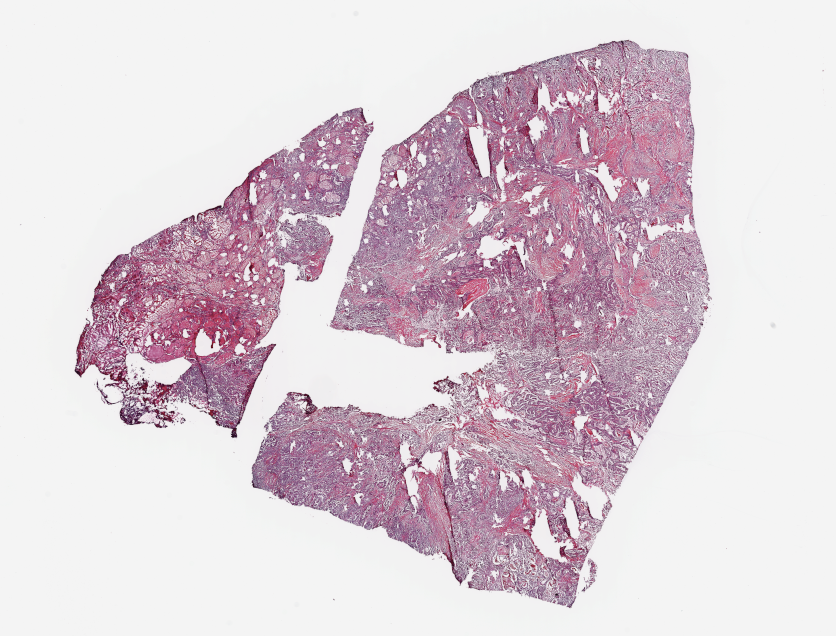
\includegraphics[width=\linewidth]{figs/introduction/Sample_WSI.PNG}
    \end{center}
    \caption{نمونه اسلاید اسکن شده از غده تیروئید}
    \label{fig:sampleWSIscan}
\end{figure}
این اسلاید ها معمولا ابعاد بسیار بزرگی دارند و ممکن است تا بزرگنمایی 40 برابر را پشتیبانی کنند.
به همین دلیل ممکن است حجمی بین چند مگابایت تا چند گیگابایت را به خود بگیرند.

مدل هوش مصنوعی که در این پژوهش توسعه داده می شود، باید قادر باشد ویژگی های سلول ها را از روی این اسلاید ها تشخیص داده و تخمین درستی از وضعیت سرطان به ما بدهد.



\section{شبکه عصبی پیچشی و یادگیری عمیق}\label{sec:شبکه عصبی پیچشی و یادگیری عمیق}
شبکه عصبی پیچشی\LTRfootnote{Convolutional Neural Network} یک معماری یادگیری عمیق\LTRfootnote{Deep Learning} است که می‌تواند یک تصویر ورودی را گرفته، به جنبه‌ها یا اشیای مختلف آن تصویر از طریق وزن‌دهی قابل یادگیری، اهمیت بخشد و بتواند یکی را از دیگری متمایز کند. معماری شبکه‌های عصبی پیچشی مشابه الگوی اتصال نورون‌ها در مغز انسان است و از ساختار قشر بصری الهام گرفته است.

معماری شبکه عصبی پیچشی ابتدا در سال 2015 و در مقاله \cite{o2015introduction} معرفی شد که در تصویر \ref{fig:cnnarchitecture} آمده است. ساختار کلی آن، از تعدادی لایه‌های پیچشی تشکیل شده است که در هر لایه تعدادی کانال وجود دارد که هر کدام به طور مستقل از ماتریس‌های هسته آن لایه و خروجی لایه قبل بوجود می‌آیند.
\begin{figure}
    \begin{center}
        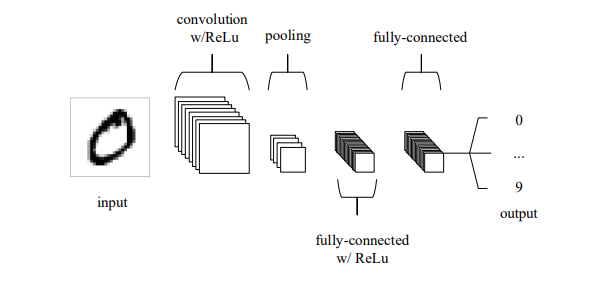
\includegraphics[width=0.8\linewidth]{figs/basic_concepts/subs/cnn_image_processing/basic_cnn_arhitecture.PNG}
    \end{center}
    \caption{ساختار پایه معماری شبکه عصبی پیچشی}
    \label{fig:cnnarchitecture}
\end{figure}

عملکرد این معماری برای گروه‌بندی تصاویر در بسیاری از موارد بالا است و شبکه‌هایی با این معماری وجود دارند که در پردازش تصویر به دقت انسان‌ها رسیده و حتی در مواردی دقتی بیشتر از انسان را داشته‌اند. به همین دلیل در سال‌های اخیر، معماری پایه‌ی بسیاری از پژوهش‌ها است.
این معماری پایه‌ی بسیاری از شبکه‌های عصبی دیگر برای پردازش تصویر است.
